\chapter{Nimplex Workshop No.2 - Additive Manufacturing Path Planning Made
Effortless} \label{chap:nimplextutorial2}

This is the second tutorial going over basics of use of the \texttt{nimplex} software. It goes over its core advantages in additive manufacturing and can be run on the cloud using pre-compiled virtual environment following the current Quick Start link at \href{https://nimplex.phaseslab.org}{nimplex.phaseslab.org}.

\section{Introduction}

In this tutorial, we will demonstrate how effortless it is to
dramatically speed up the exploration of feasible compositional spaces
in high dimensional spaces through employing
\texttt{nimplex}'s graph representations that abstract
the underlying problem and dimensionality.

We will also design several neat, mathematically optimal (given
some criteria) paths in a 7-component chemical space connecting two
alloys of interest by mixing 4 fixed-composition alloy powders to create
a tetrahedral attainable/design space. The beauty of this approach is
that at no point (except for plotting in 3D for ``human consumption'')
will we explicitly consider the dimensionality or the distance as the
connectivity between the points in the space has been abstracted into
graph adjacency. If you wish to add another alloy to the design process,
you add it to the list, and you are done!

\begin{minted}[xleftmargin=3\parindent, linenos=true, fontsize=\small]{python}
# Import nimplex and some of its plotting utilities.
import nimplex
from utils import plotting
\end{minted}

\begin{minted}[xleftmargin=3\parindent, linenos=true, fontsize=\small]{python}
# Python wrapper for Plotly library
import plotly.express as px
import plotly.io as pio
pio.renderers.default = 'pdf'
import pandas as pd
from pprint import pprint
\end{minted}

\section{Recall Last Example}\label{nimplextutorial2:recall-last-example}

Let's get back to our example (QuickStart) of the pair of
\textbf{attainable space} simplex grid and corresponding
\textbf{elemental space} positions defined for
\texttt{7}-component elemental space of
\texttt{Ti}, \texttt{Zr},
\texttt{Hf}, \texttt{W},
\texttt{Nb}, \texttt{Ta}, and
\texttt{Mo} formed by \texttt{4}
alloys: - Ti50 Zr50 - Hf95 Ti5 - Mo33 Nb33 Ta33 - Mo10 Nb10 W80

which we can represent as points in the elemental space:

\begin{minted}[xleftmargin=3\parindent, linenos=true, fontsize=\small]{python}
elementalSpaceComponents = 
  ["Ti", "Zr", "Hf", "W", "Nb", "Ta", "Mo"]
attainableSpaceComponents = 
  ["Ti50 Zr50", "Hf95 Ti5", "Mo33 Nb33 Ta33", "Mo80 Nb10 W10"]
attainableSpaceComponentPositions = 
  [[50, 50, 0, 0, 0, 0, 0], [5, 0, 95, 0, 0, 0, 0], 
  [0, 0, 0, 33, 33, 33, 0], [0, 0, 0, 10, 10, 0, 80]]
\end{minted}

And create tetrahedral grids with their compositions quantized at
\texttt{12} divisions per dimension.

\begin{minted}[xleftmargin=3\parindent, linenos=true, fontsize=\small]{python}
gridAtt, gridEl =
  nimplex.embeddedpair_simplex_grid_fractional_py(
    attainableSpaceComponentPositions, 12)
\end{minted}

We used the \textbf{elemental}, or chemical, space to run the Root Mean
Square Atomic Displacement (RMSAD) model by Tandoc
(10.1038/s41524-023-00993-x) which acts as a lower-cost proxy for yield
stress and hardness estimations in the absence of direct data:

\begin{minted}[xleftmargin=3\parindent, linenos=true, fontsize=\small]{python}
import pqam_rmsadtandoc2023
rmsadList = []
for point in gridEl:
    formula = ' '.join(
      [f'{c}{p}' for c, p in zip(elementalSpaceComponents, point)])
    rmsadList.append(pqam_rmsadtandoc2023.predict(formula))
\end{minted}

And the \textbf{attainable} space grid to plot the results after
projecting them to the Euclidean space:

\begin{minted}[xleftmargin=3\parindent, linenos=true, fontsize=\small]{python}
# Hover approximate formula for each point
formulas = []
for i, comp in enumerate(gridEl):
    formulas.append(f"({i:>3}) "+"".join(
      [f"{el}{100*v:.1f} " if v>0 else "" for 
        el, v in zip(elementalSpaceComponents, comp)]))

# Generate the projected grid
gridAtt_projected_df = 
  pd.DataFrame(plotting.simplex2cartesian_py(gridAtt), columns=['x','y','z'])

# Attach pure component (alloy) labels to corners
pureComponentIndices = nimplex.pure_component_indexes_py(4, 12)
labels = ['']*len(gridAtt_projected_df)
for comp, idx in zip(attainableSpaceComponents, pureComponentIndices):
    labels[idx] = "<b>"+comp+"</b>"

# Add text labels at the corners of the simplex
px.scatter_3d(
  gridAtt_projected_df, x='x', y='y', z='z', 
  color=rmsadList, text=labels, hover_name=formulas,
  template='plotly_white', width=800, height=700, 
  labels={'color':'RMSAD', 'x':'', 'y':'', 'z':''})
\end{minted}

\begin{figure}[H]
    \centering
    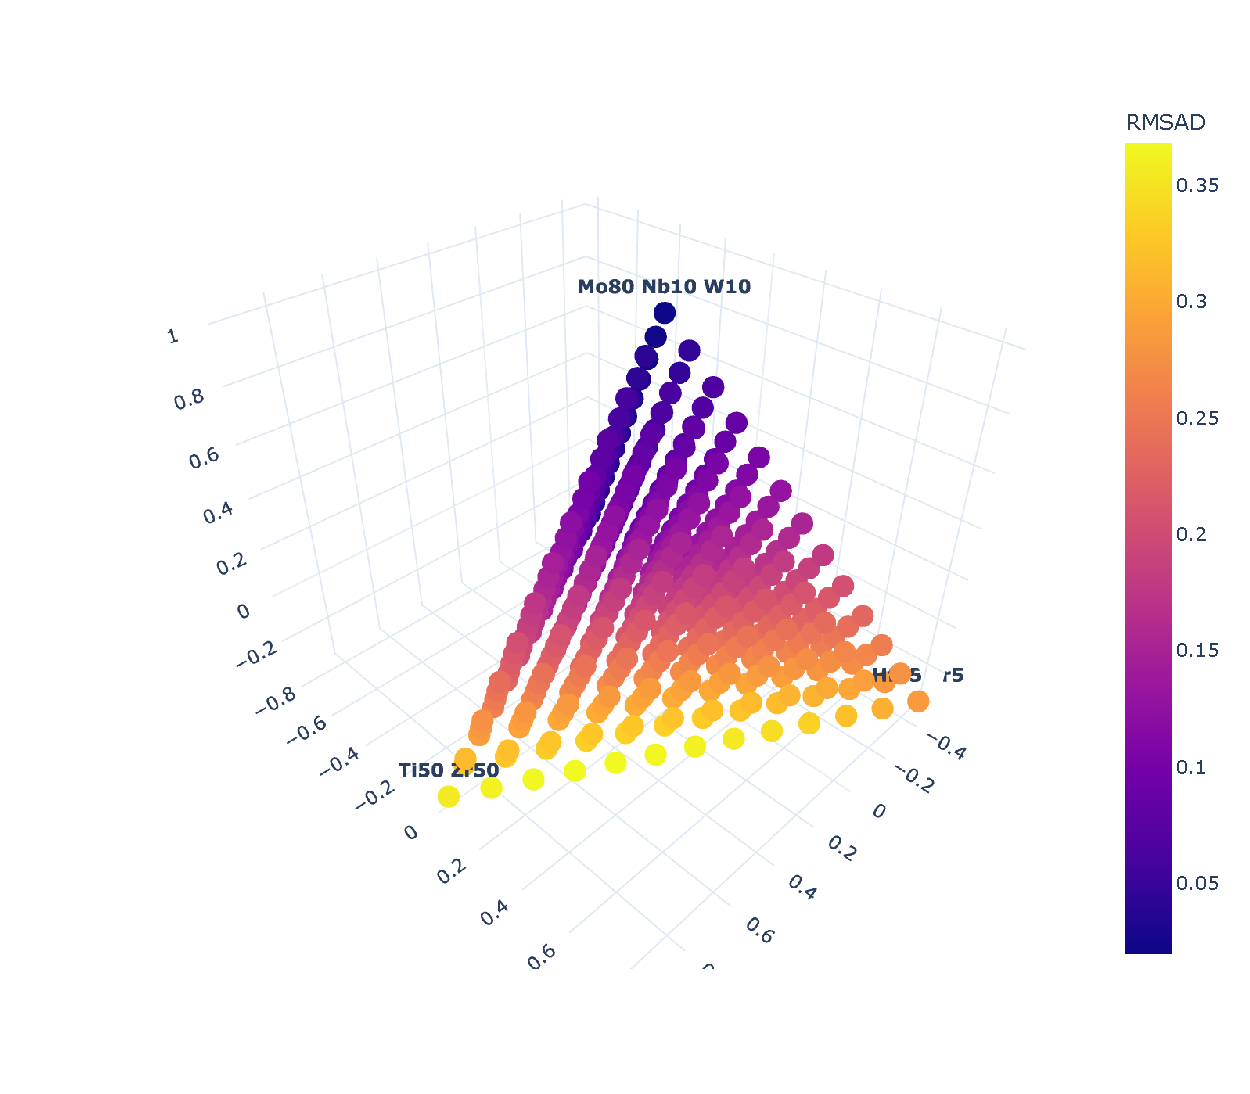
\includegraphics[width=0.8\textwidth]{nimplextutorial2/02.AdditiveManufacturingPathPlanning_11_0.pdf}
    \caption{Re-rendering of Figure \ref{nimplextutorial1:fig:quaternaryattainablecoloredlabel} from Appendix \ref{chap:nimplextutorial1}.}
    \label{nimplextutorial2:fig:propertyfield}
\end{figure}

\section{Thermodynamic Equilibria}\label{nimplextutorial2:thermodynamic-equilibria}

\textbf{In this section we will be using
\texttt{pycalphad} which is an amazing free open-source
library for building thermodynamic models and performing calculations on
them, including studying of phase equilibria, or what atomic
arrangements are stable (coexist in equilibrium) at a given temperature
and composition.} You can read more about
\texttt{pycalphad} at
\href{https://pycalphad.org/}{pycalphad.org} and find an great tutorial
at
\href{https://github.com/materialsgenomefoundation/2023-workshop-material/tree/main/pycalphad}{this
2023 workshop materials repository}.

Let's start by loading a database of thermodynamic properties which
defines, among other things, the Gibbs energy of each phase as a
function of temperature and composition. You can find many of such
databases at \href{https://avdwgroup.engin.brown.edu}{TDBDB} maintained
by Axel van de Walle's group at Brown University.

In this example, we will be using a TDB
\texttt{CrHfMoNbTaTiVWZr\_9element\_Feb2023} placed for
you in the \texttt{examples} directory, which is a
9-element database for the elements \texttt{Cr},
\texttt{Hf}, \texttt{Mo},
\texttt{Nb}, \texttt{Ta},
\texttt{Ti}, \texttt{V},
\texttt{W}, and \texttt{Zr}, being
developed by Shuang Lin in our group (Phases Research Lab at PSU). This
wersion is an older \emph{work in progress} one that has not been
published, so while it is perfect for tutorial like this one, please
refrain from using it for any serious work.

\begin{minted}[xleftmargin=3\parindent, linenos=true, fontsize=\small]{python}
from pycalphad import Database
dbf = Database("CrHfMoNbTaTiVWZr_9element_Feb2023.tdb")
phases = list(set(dbf.phases.keys()))
print(elementalSpaceComponents)
print(f'Loaded TDB file with phases considered: {phases}')
\end{minted}

\begin{minted}[xleftmargin=3\parindent, fontsize=\small, bgcolor=subtlegray]{output}
['Ti', 'Zr', 'Hf', 'W', 'Nb', 'Ta', 'Mo']
Loaded TDB file with phases considered: 
['LAVES_C14', 'BCC_A2', 'HCP_A3', 'LAVES_C15', 'LIQUID', 'LAVES_C36', 'FCC_A1']
\end{minted}

As you can see, we will be looking at several different phases here. To
keep things as simple as possible, we can split them in three groups: -
\textbf{liquid} phases: \texttt{LIQUID} (which we
obviously want to avoid in a solid part design) - \textbf{solid
solution} phases: \texttt{FCC\_A1},
\texttt{BCC\_A2}, and \texttt{HCP\_A3}
- \textbf{intermetallic} phases: \texttt{LAVES\_C14},
\texttt{LAVES\_C15}, and
\texttt{LAVES\_C36}

Designing an alloy is a complex procedure but for the sake of this
tutorial, we will be focusing on the most common issue which is the
formation of intermetallic phases which cause embrittlement and reduce
the ductility of the material. \textbf{Thus, we will apply a simple
constraint that the alloy should only contain the solid solution phases
FCC, BCC, and HCP.}

\textbf{Now, knowing what we are looking for (phases at equilibrium), we
can start by writing a short Python script around
\texttt{pycalphad} to calculate the equilibrium phases
for a given chemical elements composition \texttt{elP}.
It is already placed in the \texttt{examples} directory
as \texttt{myPycalphadCallable.py} which defines a
function \texttt{equilibrium\_callable} that takes a
composition and returns the equilibrium phases.}

\textbf{We will arbitrarily pick \texttt{1000K}} as the
temperature for the sake of this tutorial, but you can change it to any
other value you like. Or even make it a list and add phases present at
each temperature to a set to apply our constraint over a range of
temperatures.

Please note that much more information is generated in the process
(e.g., chemical composition of each phase and its fraction) but we are
only interested in the phase presence. If you wish to do so, modifying
the script to, e.g., allow for up to 5\% of intermetallic phases, is a
trivial task. Advanced users may also want to have a look at the
\texttt{scheil\_callable} we do not use in this
tutorial for the sake of runtime, but which can be used to simulate
solidification of the alloy from a liquid state in an additive
manufacturing process.

\begin{minted}[xleftmargin=3\parindent, linenos=true, fontsize=\small]{python}
from myPycalphadCallable import equilibrium_callable
\end{minted}

Let's test it on some composition in our space starting with the first
point!

\begin{minted}[xleftmargin=3\parindent, linenos=true, fontsize=\small]{python}
print(formulas[0])
equilibrium_callable(gridEl[0])
\end{minted}

\begin{minted}[xleftmargin=3\parindent, fontsize=\small, bgcolor=subtlegray]{output}
(  0) W10.0 Nb10.0 Mo80.0 
['BCC_A2']
\end{minted}

You should see \texttt{['BCC\_A2']} in a second or so
if you've run it at the default \texttt{1000K}. Quick
and neat, right? Now, let's pick some compositionally complex alloy that
does not lay around the corner of the attainable space tetrahedron and
presents an actual challenge.

\begin{minted}[xleftmargin=3\parindent, linenos=true, fontsize=\small]{python}
print(formulas[63])
equilibrium_callable(gridEl[63])
\end{minted}

\begin{minted}[xleftmargin=3\parindent, fontsize=\small, bgcolor=subtlegray]{output}
( 63) Ti2.5 Hf47.5 W5.0 Nb5.0 Mo40.0 
['HCP_A3', 'LAVES_C15', 'BCC_A2']
\end{minted}

Now, you should have seen an example of infeasible point composed of
\texttt{['HCP\_A3', 'LAVES\_C15', 'BCC\_A2']}. Let's
deploy this in parallel over all the points in the elemental space
\texttt{gridEl} and see how it looks like! We will use
the \texttt{process\_map} function from the
\texttt{tqdm} library to show a neat progress bar while
the calculations are running in parallel. On the 4-core Codespaces VM
you can expect it to take around 2-3 minutes.

\begin{minted}[xleftmargin=3\parindent, linenos=true, fontsize=\small]{python}
from tqdm import tqdm
from tqdm.contrib.concurrent import process_map
\end{minted}

\begin{minted}[xleftmargin=3\parindent, linenos=true, fontsize=\small]{python}
gridPhases = process_map(equilibrium_callable, gridEl)
\end{minted}

\begin{minted}[xleftmargin=3\parindent, fontsize=\small, bgcolor=subtlegray]{output}
  0%|          | 0/455 [00:00<?, ?it/s]
\end{minted}

Let's see how some of the data looks like.

\begin{minted}[xleftmargin=3\parindent, linenos=true, fontsize=\small]{python}
gridPhases[120:130]
\end{minted}

\begin{minted}[xleftmargin=3\parindent, fontsize=\small, bgcolor=subtlegray]{output}
[['HCP_A3', 'BCC_A2', 'LAVES_C15'],
 ['HCP_A3', 'BCC_A2'],
 ['HCP_A3', 'BCC_A2'],
 [],
 ['LAVES_C15', 'BCC_A2'],
 ['LAVES_C15', 'BCC_A2', 'HCP_A3'],
 ['HCP_A3', 'LAVES_C15', 'BCC_A2'],
 ['LAVES_C15', 'HCP_A3', 'BCC_A2'],
 ['HCP_A3', 'BCC_A2', 'LAVES_C15'],
 ['HCP_A3', 'BCC_A2', 'LAVES_C15']]
\end{minted}

Now, let's turn that list of phases into a list of feasibility based on
the constraint we defined earlier. Note that in some cases, the
\texttt{pycalphad} library may return an empty list of
phases, which we will treat as infeasible.

\begin{minted}[breaklines, xleftmargin=3\parindent, linenos=true, fontsize=\small]{python}
gridFeasible = 
  [len(set(p) & set(['LAVES_C15', 'LAVES_C36', 'LAVES_C14', 'LIQUID']))==0 and p!=[] for p in gridPhases]
gridFeasible[120:130]
\end{minted}

\begin{minted}[xleftmargin=3\parindent, fontsize=\small, bgcolor=subtlegray]{output}
[False, True, True, False, False, False, False, False, False, False]
\end{minted}

Finally, let's plot the result in 3D using the
\texttt{plotly} library and our spacial-transformed
attainable space grid we obtained with
\texttt{plotting.simplex2cartesian\_py(gridAtt)}
earlier.

\textbf{Once you run the cell below, you should be seeing an interactive
3D plot with 455 split roughly 50/50 between feasible and infeasible
points. You can rotate the plot, zoom in and out, and hover over the
points to see their composition and feasibility. You can also click on
the legend to hide/show the points based on their feasibility.}

\begin{minted}[xleftmargin=3\parindent, linenos=true, fontsize=\small]{python}
fig = px.scatter_3d(
  gridAtt_projected_df, x='x', y='y', z='z', color=gridFeasible, 
  text=labels, hover_name=formulas, template='plotly_white', 
  width=800, height=700, opacity=0.333, 
  color_discrete_sequence=['green', 'red'], 
  labels={'color':'Solid Solution Phases', 'x':'', 'y':'', 'z':''})
fig.update_scenes({'camera': {'eye': {'x': -2.3, 'y': 0.2, 'z': 0.2}}})
\end{minted}

\begin{figure}[H]
    \centering
    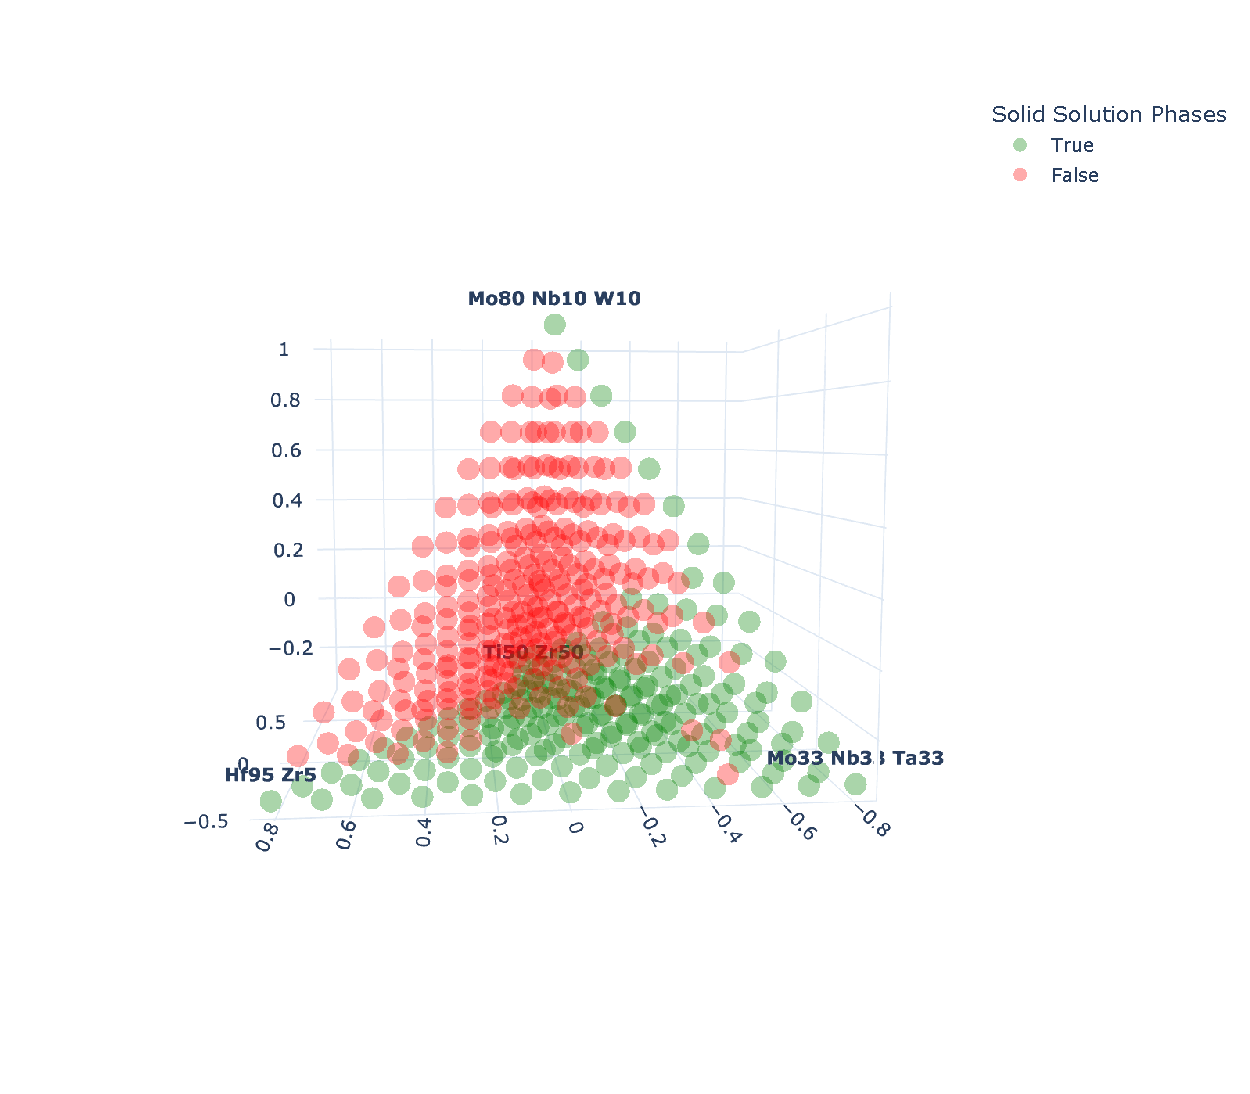
\includegraphics[width=0.8\textwidth]{nimplextutorial2/02.AdditiveManufacturingPathPlanning_28_1.pdf}
    \caption{Feasibility map constrained by limiting phases present at equilibrium at 1000K to single or many solid solution phases demonstrating roughly half of the system to be infeasible.}
    \label{nimplextutorial2:fig:fullfeasibility}
\end{figure}


\section{Graph Walk aka Infeasibility Gliding (Exciting
Stuff!)}\label{nimplextutorial2:graph-walk-aka-infeasibility-gliding-exciting-stuff}

\textbf{While the last two sections highlighted the elegant abstraction
of grid generation and space transformation using
\texttt{nimplex}, they did not really show the true
power of the library or the novel combinatorics-based algorithm we
developed in the associated paper. That is the simplex graph
construction in arbitrary dimensions and the graph traversal it
enables.}

\textbf{Let's start by generating the graph for our problem. We can use
the function called
\texttt{nimplex.embeddedpair\_simplex\_graph\_fractional\_py}, which also first generates the two grids we already used in
the previous sections.}

\begin{minted}[xleftmargin=3\parindent, linenos=true, fontsize=\small]{python}
_, _, graphN = 
  nimplex.embeddedpair_simplex_graph_fractional_py(
    attainableSpaceComponentPositions, 12)
\end{minted}

As you can see, we immediately obtain list of adjecent nodes
(compostions) for each node in the graph, with few neighbors for the
corners and many for the interior points. This is the power of the
abstraction we are talking about!

\begin{minted}[xleftmargin=3\parindent, linenos=true, fontsize=\small]{python}
graphN[:5]
\end{minted}

\begin{minted}[xleftmargin=3\parindent, fontsize=\small, bgcolor=subtlegray]{output}
[[1, 13, 91],
 [0, 2, 13, 14, 91, 92],
 [1, 3, 14, 15, 92, 93],
 [2, 4, 15, 16, 93, 94],
 [3, 5, 16, 17, 94, 95]]
\end{minted}

\begin{minted}[xleftmargin=3\parindent, linenos=true, fontsize=\small]{python}
graphN[200:205]
\end{minted}

\begin{minted}[xleftmargin=3\parindent, fontsize=\small, bgcolor=subtlegray]{output}
[[134, 126, 125, 192, 191, 199, 201, 207, 208, 255, 262, 263],
 [135, 127, 126, 193, 192, 200, 202, 208, 209, 256, 263, 264],
 [136, 128, 127, 194, 193, 201, 203, 209, 210, 257, 264, 265],
 [137, 129, 128, 195, 194, 202, 204, 210, 211, 258, 265, 266],
 [138, 130, 129, 196, 195, 203, 205, 211, 212, 259, 266, 267]]
\end{minted}

We can now use this graph to do a lot of things. Let's start by
considering that \textbf{the infeasible region, for thermodynamic
reasons beyond the scope of this tutorial, are generally difficult to
predict but are generally bound by continous surfaces called phase
boundaries.}

\textbf{Thus, if we iteratively traverse the graph expanding only the
feasible nodes, while noting infeasible nodes, we can glide along the
phase boundaries and explore the feasible space without ever wasting our
resources on calculations inside the insides of the infeasible regions.}

Let's do this starting from the
\texttt{W10.0 Nb10.0 Mo80.0} and terminating when we
reach the \texttt{Hf95.0 Ti5.0} point.

\textbf{Bonus Exercises:} - Please note that you do not need to specify
the termination point, as the algorithm will stop when it completeley
explores the feasible space. In this example, we are just showing you
how to specify it and it has no effect on the result. If you want to
play a bit, you can set \texttt{endNode} to
\texttt{12} to see how path to
\texttt{W33.3 Nb33.3 Ta33.3} gets explored in just 87
nodes. - If you remove the \texttt{endNode} termination
(change \texttt{break} to
\texttt{pass}), you can add the endNode (or any other
node you believe is feasible) to the initial
\texttt{queue} list and see how the algorithm explores
the feasible space from multiple starting points much faster thanks to
better parallelization.

\begin{minted}[xleftmargin=3\parindent, linenos=true, fontsize=\small]{python}
startingNode = 0
endNode = 90

print(f"Starting node: {formulas[startingNode]}")
print(f"Ending node: {formulas[endNode]}")
\end{minted}

\begin{minted}[xleftmargin=3\parindent, fontsize=\small]{output}
Starting node: (  0) W10.0 Nb10.0 Mo80.0 
Ending node: ( 90) Ti5.0 Hf95.0 
\end{minted}

\begin{minted}[xleftmargin=3\parindent, linenos=true, fontsize=\small]{python}
gridFeasible = [None]*len(graphN)
queue = [startingNode]
explored = set()
calcCount = 0
\end{minted}

\textbf{Now, we will be using a \texttt{queue} of nodes
to keep track of the nodes we need to visit and a set of visited nodes
to avoid revisiting them. This simple procedure is a type of
\texttt{depth-first search} algorithm that is
guaranteed to find the shortest path between two points in a graph if it
exists, while exploring the feasible space in the process in an unbiased
way. In a more elaborate problem, you would likely want to implement a
priority queue to explore the space in a more efficient way, but for
this tutorial, this is more than enough and allows for better, more
direct comparions with the typical complete exploration approach.} On
the 4-core Codespaces VM you can expect it to take around 1-2 minutes.
In a relatively simple problem like this one, the difference between the
two approaches is not that big, coming partially from overhead of
limited Python parallelization capabilities, but in a more complex
problem, the difference can be dramatic.

\begin{minted}[breaklines, xleftmargin=3\parindent, linenos=true, fontsize=\small]{python}
while len(queue)>0:
    print(f"Queue: {queue}")
    # Assign feasibilities to the current queue
    elPositions = [gridEl[i] for i in queue]
    if len(queue)>3:
        phases = process_map(
          equilibrium_callable, elPositions, max_workers=4)
    else:
        phases = [equilibrium_callable(elP) for elP in elPositions]
    feasibilities = [len(set(p) & set(['LAVES_C15', 'LAVES_C36', 'LAVES_C14', 'LIQUID']))==0 and p!=[] for p in phases]

    calcCount += len(feasibilities)
    explored = explored.union(queue)

    # Create next queue based on neighbors of feasible points
    nextQueue = set()
    for f, i in zip(feasibilities, queue):
        gridFeasible[i] = f
        # Only if feasible
        if f:
            for n in graphN[i]:
                if n not in explored:
                    nextQueue.add(n)

    # Early termination criteria if we just evaluated the target
    if endNode in queue:
        break

    print(f"Calculations done: {calcCount}")
    queue = list(nextQueue)
\end{minted}

\begin{minted}[xleftmargin=3\parindent, fontsize=\small, bgcolor=subtlegray]{output}
Queue: [0]
Calculations done: 1
Queue: [1, 91, 13]
Calculations done: 4
Queue: [2, 92, 14]
...
Calculations done: 87
Queue: [129, 132, 261, 138, 139, 266, 267, 268, 140, 12, 24, 35, 42, 298, 44, 
45, 306, 179, 52, 53, 311, 312, 313, 189, 198, 203, 206, 211, 212, 213, 342, 
346, 347, 348, 349, 102, 113, 244, 374, 375, 376, 377, 123, 253]
  0%|          | 0/44 [00:00<?, ?it/s]
Calculations done: 131
Queue: [273, 146, 147, 274, 401, 402, 403, 404, 54, 310, 317, 62, 61, 318, 319, 
218, 219, 353, 354, 355, 373, 380, 381, 382, 383]
  0%|          | 0/25 [00:00<?, ?it/s]
Calculations done: 156
...
Queue: [396, 398, 287, 289, 417, 419, 164, 167, 434, 444, 450, 453, 454, 332, 
334, 83, 87, 232, 234, 368, 370]
  0%|          | 0/21 [00:00<?, ?it/s]
Calculations done: 277
Queue: [168, 89, 166, 86]
  0%|          | 0/4 [00:00<?, ?it/s]
Calculations done: 281
Queue: [88, 90]
\end{minted}

\textbf{You should now see that only 281 phase equilibria calculations
were performed to get all the feasible points! That's only a bit more
than half of what we had to do in the previous section. Let's plot the
path we found in the 3D space.} If you rotate the figure, you can
clearly see the path gliding along the infeasible space boundary.

\begin{minted}[breaklines, xleftmargin=3\parindent, linenos=true, fontsize=\small]{python}
fig = px.scatter_3d(
  gridAtt_projected_df, x='x', y='y', z='z', color=gridFeasible, 
  text=labels, hover_name=formulas, template='plotly_white', 
  width=800, height=700, opacity=0.333, 
  color_discrete_sequence=['green', 'red'], 
  labels={'color':'Solid Solution Phases', 'x':'', 'y':'', 'z':''})
fig.update_scenes({'camera': {'eye': {'x': -2.3, 'y': 0.2, 'z': 0.2}}})
\end{minted}

\begin{figure}[H]
    \centering
    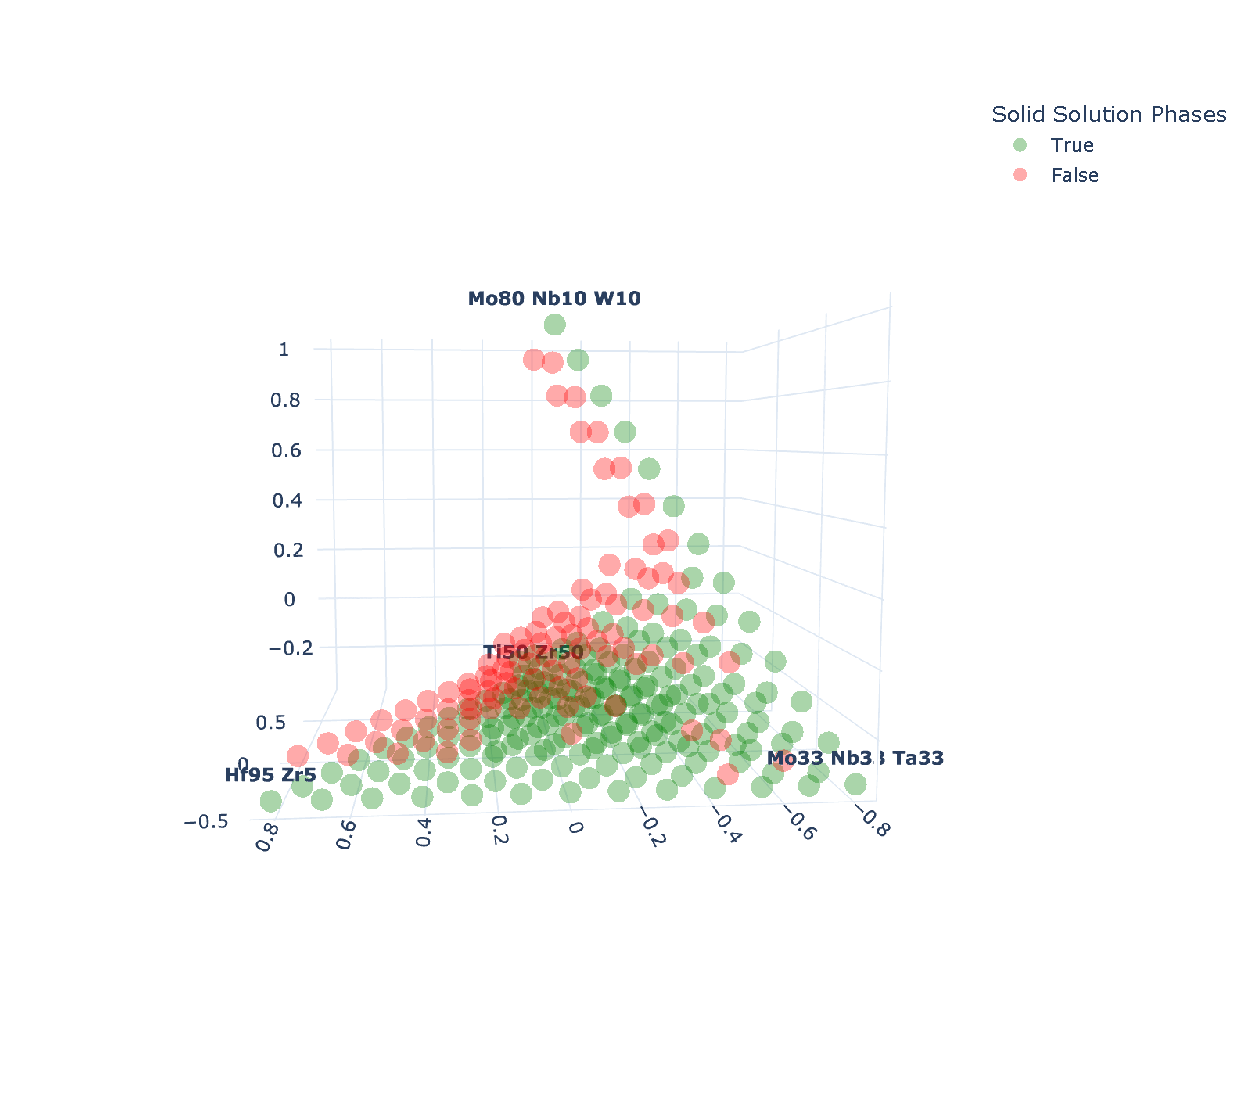
\includegraphics[width=0.8\textwidth]{nimplextutorial2/02.AdditiveManufacturingPathPlanning_40_1.pdf}
    \caption{Feasibility map created by gliding over the infeasible region boundary, efficiently calculating all feasible points at the minimum number of evaluations.}
    \label{nimplextutorial2:fig:infeasibilityglide}
\end{figure}

\section{Path Finding}\label{nimplextutorial2:path-finding}

\textbf{Now, let's take the appeal of graph representation a few steps
forward! Since they are very general and widely applicable, there are
countless off-the-shelf high-performance libraries implementing
mathematically optimal path finding algorithms on graphs one can deploy
on challenging problems.}

In this example, for the sake of simplicity, we will use pure-Python
\texttt{pathfinding} library which implements some of
the most popular path finding algorithms without high performance (we do
not need here) but also without any dependencies. In real applications,
you would likely want to use a more advanced library like
\texttt{networkx} which is more efficient and have more
features, or write one yourself. Please note that
\texttt{nimplex}'s CLI can generate massive graphs in
native NumPy format you may find useful for such applications (e.g., to
use Julia or C++ libraries).

\begin{minted}[xleftmargin=3\parindent, linenos=true]{python}
from pathfinding.core.graph import Graph
from pathfinding.finder.dijkstra import DijkstraFinder
\end{minted}

Let's now turn our graph definition into a format that
\texttt{pathfinding} library can understand, assigning
equal cost to all edges. \textbf{Note, that we only need to consider the
feasible points leading to other feasible point}

\begin{minted}[breaklines, xleftmargin=3\parindent, linenos=true, fontsize=\small]{python}
edges = []
for i, nList in enumerate(graphN):
    if gridFeasible[i]:
        for n in nList:
            if gridFeasible[n]:
                edges.append([i, n, 1])
print(edges[:5])
\end{minted}

\begin{minted}[xleftmargin=3\parindent, fontsize=\small, bgcolor=subtlegray]{output}
[[0, 1, 1], [1, 0, 1], [1, 2, 1], [2, 1, 1], [2, 3, 1]]
\end{minted}

Let's initialize the \texttt{Graph} object.

\begin{minted}[breaklines, xleftmargin=3\parindent, linenos=true, fontsize=\small]{python}
pathfindingGraph = Graph(edges=edges, bi_directional=False)
\end{minted}

Now, let's create the \texttt{Finder} object that will
perform the path finding. Here we use the
\texttt{DijkstraFinder} which is a very popular
algorithm for path finding in graphs (see
\href{https://en.wikipedia.org/wiki/Dijkstra's_algorithm}{it's Wikipedia
page} for more details). It \textbf{finds the shortest possible path
between two points in the graph}, which is exactly what we need here. In
the future tutorials, we will use some more advanced algorithms, like
A*, which accomplishes the same task but in the mathematcally minimal
number of evaluations.

\begin{minted}[breaklines, xleftmargin=3\parindent, linenos=true, fontsize=\small]{python}
finder = DijkstraFinder()
\end{minted}

For hundreds of points, this shouldn't take more than tenth of a second
or so.

\begin{minted}[breaklines, xleftmargin=3\parindent, linenos=true, fontsize=\small]{python}
path, runs = finder.find_path(
    pathfindingGraph.node(0), 
    pathfindingGraph.node(90), 
    pathfindingGraph)
\end{minted}

Let's now turn the path into a list of nodes on the path.

\begin{minted}[breaklines, xleftmargin=3\parindent, linenos=true, fontsize=\small]{python}
shortestPath = [p.node_id for p in path]
\end{minted}

And plot corresponding compositions. As you can see, we immediately get
a neat list of compositions that we can use to design our additive
manufacturing path.

\begin{minted}[breaklines, xleftmargin=3\parindent, linenos=true, fontsize=\small]{python}
for step, i in enumerate(shortestPath):
    print(f"{step+1:>2}: {formulas[i]}")
\end{minted}

\begin{minted}[xleftmargin=3\parindent, fontsize=\small, bgcolor=subtlegray]{output}
 1: (  0) W10.0 Nb10.0 Mo80.0 
 2: (  1) W11.9 Nb11.9 Ta2.8 Mo73.3 
 3: (  2) W13.9 Nb13.9 Ta5.6 Mo66.7 
 4: (  3) W15.8 Nb15.8 Ta8.3 Mo60.0 
 5: (  4) W17.8 Nb17.8 Ta11.1 Mo53.3 
 6: (  5) W19.7 Nb19.7 Ta13.9 Mo46.7 
 7: (  6) W21.7 Nb21.7 Ta16.7 Mo40.0 
 8: (  7) W23.6 Nb23.6 Ta19.4 Mo33.3 
 9: ( 98) Ti4.2 Zr4.2 W22.8 Nb22.8 Ta19.4 Mo26.7 
10: (110) Ti4.6 Zr4.2 Hf7.9 W21.9 Nb21.9 Ta19.4 Mo20.0 
11: (121) Ti5.0 Zr4.2 Hf15.8 W21.1 Nb21.1 Ta19.4 Mo13.3 
12: ( 43) Ti1.2 Hf23.8 W21.1 Nb21.1 Ta19.4 Mo13.3 
13: ( 53) Ti1.7 Hf31.7 W20.3 Nb20.3 Ta19.4 Mo6.7 
14: ( 61) Ti2.1 Hf39.6 W17.5 Nb17.5 Ta16.7 Mo6.7 
15: ( 68) Ti2.5 Hf47.5 W14.7 Nb14.7 Ta13.9 Mo6.7 
16: ( 74) Ti2.9 Hf55.4 W11.9 Nb11.9 Ta11.1 Mo6.7 
17: ( 80) Ti3.3 Hf63.3 W11.1 Nb11.1 Ta11.1 
18: ( 84) Ti3.8 Hf71.2 W8.3 Nb8.3 Ta8.3 
19: ( 87) Ti4.2 Hf79.2 W5.6 Nb5.6 Ta5.6 
20: ( 89) Ti4.6 Hf87.1 W2.8 Nb2.8 Ta2.8 
21: ( 90) Ti5.0 Hf95.0 
\end{minted}

\textbf{Even better, since we know the positions in the attainable
design space, we can get a list of exact quantized instructions (e.g.,
powder flow rates) for the additive manufacturing apparatus to follow at
each step.}

\textbf{This is a very powerful abstraction, eliminating possible
mistakes and miscommunications between design and manufacturing teams.
Furthermore, it also allows for easy manual (or mechanized) per-layer
mixing of powders to create compositional paths in single-feed additive
manufacturing systems.}

\begin{minted}[breaklines, xleftmargin=3\parindent, linenos=true, fontsize=\small]{python}
integerGrid = nimplex.simplex_grid_py(4, 12)
for step, i in enumerate(shortestPath):
    print(f"{step+1:>2}: {integerGrid[i]}")
\end{minted}

\begin{minted}[xleftmargin=3\parindent, fontsize=\small, bgcolor=subtlegray]{output}
 1: [0, 0, 0, 12]
 2: [0, 0, 1, 11]
 3: [0, 0, 2, 10]
 4: [0, 0, 3, 9]
 5: [0, 0, 4, 8]
 6: [0, 0, 5, 7]
 7: [0, 0, 6, 6]
 8: [0, 0, 7, 5]
 9: [1, 0, 7, 4]
10: [1, 1, 7, 3]
11: [1, 2, 7, 2]
12: [0, 3, 7, 2]
13: [0, 4, 7, 1]
14: [0, 5, 6, 1]
15: [0, 6, 5, 1]
16: [0, 7, 4, 1]
17: [0, 8, 4, 0]
18: [0, 9, 3, 0]
19: [0, 10, 2, 0]
20: [0, 11, 1, 0]
21: [0, 12, 0, 0]
\end{minted}

We can also plot the path in 3D like we did before! As you can see, it
\textbf{glides through the inside of the tetrahedron in a shortest path}
avoiding an obstacle extending far on the face.

\begin{minted}[breaklines, xleftmargin=3\parindent, linenos=true, fontsize=\small]{python}
gridFeasibleMarked = ['path' if i in shortestPath else f for i, f in enumerate(gridFeasible)]
fig = px.scatter_3d(
  gridAtt_projected_df, x='x', y='y', z='z', color=gridFeasibleMarked, 
  text=labels, hover_name=formulas, template='plotly_white', width=800, 
  height=700, opacity=0.333, color_discrete_sequence=['blue', 'green', 'red'],
  labels={'color':'Solid Solution Phases', 'x':'', 'y':'', 'z':''})
fig.update_scenes({'camera': {'eye': {'x': -1.8, 'y': 1.2, 'z': 1.5}}})
\end{minted}

\begin{figure}[H]
    \centering
    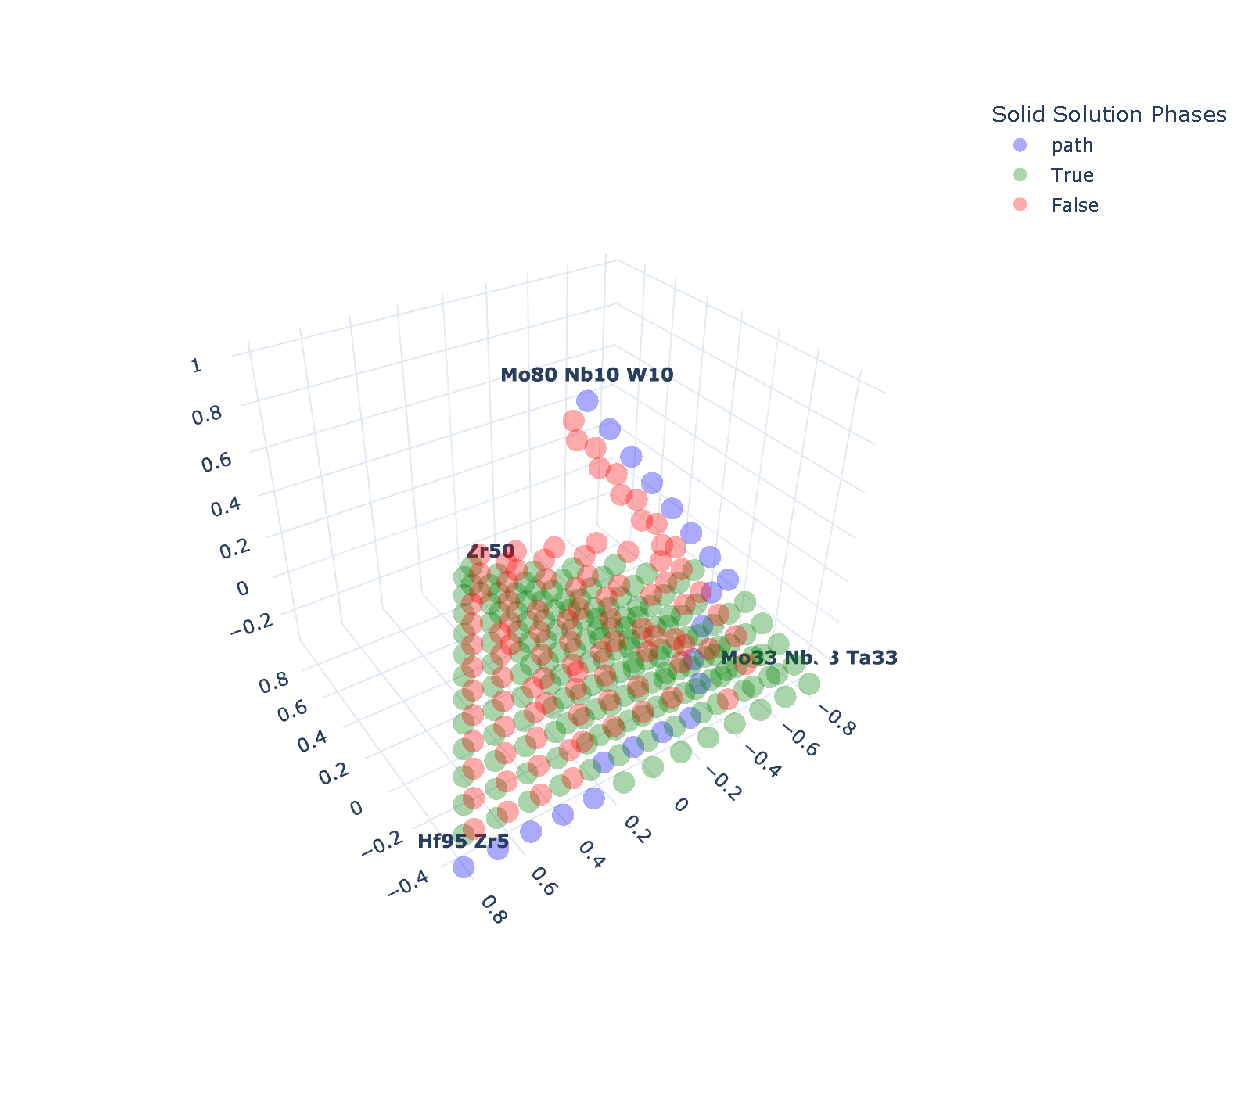
\includegraphics[width=0.8\textwidth]{nimplextutorial2/02.AdditiveManufacturingPathPlanning_58_1.pdf}
    \caption{An optimal shortest path between W10 Nb10 Mo80 and Ti5 Hf95 connecting them in 21 steps.}
    \label{nimplextutorial2:fig:shortest}
\end{figure}


\section{Path Planning considering the Property
Gradient}\label{nimplextutorial2:path-planning-considering-the-property-gradient}

\textbf{Let's go one step further to demonstrate the beaty of the graph
representations in the context of efortless path planning in
high-dimensional spaces by including the gradient into consideration in
just a line or two of code. We will now stretch the space}

\begin{minted}[breaklines, xleftmargin=3\parindent, linenos=true, fontsize=\small]{python}
edges = []
gradientsList = []
penaltyFactor = 100
for i, nList in enumerate(graphN):
    if gridFeasible[i]:
        for n in nList:
            if gridFeasible[n]:
                rmsadGradient = abs(rmsadList[i]-rmsadList[n])
                gradientsList.append(rmsadGradient)
                edges.append([i, n, 1+round(rmsadGradient*penaltyFactor, 3)])
print(edges[:5])
print(f"{len(gradientsList)} gradients calculated with absolute value range between {min(gradientsList)} to {max(gradientsList)}")
print(f"Penalty at {penaltyFactor}x gradient *magnitude* per path step assigned.")
\end{minted}

\begin{minted}[xleftmargin=3\parindent]{output}
[[0, 1, 1.2770000000000001], [1, 0, 1.2770000000000001], [1, 2, 1.232], 
[2, 1, 1.232], [2, 3, 1.208]]
1374 gradients calculated with absolute value range between 
8.898859123501746e-06 to 0.0473823732310002
Penalty at 100x gradient *magnitude* per path step assigned.
\end{minted}

\textbf{As you can see, we just increased the predicted cost of moving
between nodes by a small factor ranging from near 0 to 2.5 depending on
the RMSAD gradient. In another words, we are prioritizing paths that
change RMSAD the least over the entire path.} This can be done, e.g., to
minimize the inter-layer stresses in the component caused by yield
stress mismatch between the layers that may cause delamination. Similar
considerations can also be made for other properties, like thermal
expansion coefficient, missmatch of which causes internal stress or
wrapping.

\textbf{Since the RMSAD is generally smoothly changing, we can expect
that this will not impact the result in terms of number of nodes. Just
finding a better path of equivalent length. However, if you try to
square the gradient by changing penalty to
\texttt{(rmsadGradient*penaltyFactor)**2}, you will see
how viciously the path will avoid any RMSAD changes through zig-zag
patterns.}

\begin{minted}[breaklines, xleftmargin=3\parindent, linenos=true, fontsize=\small]{python}
pathfindingGraph = Graph(edges=edges, bi_directional=False)
finder = DijkstraFinder()
path, runs = finder.find_path(
    pathfindingGraph.node(0), 
    pathfindingGraph.node(90), 
    pathfindingGraph)
lowGradientPath = [p.node_id for p in path]
\end{minted}

\begin{minted}[breaklines, xleftmargin=3\parindent, linenos=true, fontsize=\small]{python}
for step, i in enumerate(lowGradientPath):
    print(f"{step+1:>2}: {formulas[i]}")
\end{minted}

\begin{minted}[xleftmargin=3\parindent, fontsize=\small, bgcolor=subtlegray]{output}
 1: (  0) W10.0 Nb10.0 Mo80.0 
 2: (  1) W11.9 Nb11.9 Ta2.8 Mo73.3 
 3: (  2) W13.9 Nb13.9 Ta5.6 Mo66.7 
 4: (  3) W15.8 Nb15.8 Ta8.3 Mo60.0 
 5: (  4) W17.8 Nb17.8 Ta11.1 Mo53.3 
 6: (  5) W19.7 Nb19.7 Ta13.9 Mo46.7 
 7: (  6) W21.7 Nb21.7 Ta16.7 Mo40.0 
 8: ( 97) Ti4.2 Zr4.2 W20.8 Nb20.8 Ta16.7 Mo33.3 
 9: (175) Ti8.3 Zr8.3 W20.0 Nb20.0 Ta16.7 Mo26.7 
10: (186) Ti8.8 Zr8.3 Hf7.9 W19.2 Nb19.2 Ta16.7 Mo20.0 
11: (196) Ti9.2 Zr8.3 Hf15.8 W18.3 Nb18.3 Ta16.7 Mo13.3 
12: (205) Ti9.6 Zr8.3 Hf23.8 W17.5 Nb17.5 Ta16.7 Mo6.7 
13: (139) Ti5.8 Zr4.2 Hf31.7 W17.5 Nb17.5 Ta16.7 Mo6.7 
14: ( 61) Ti2.1 Hf39.6 W17.5 Nb17.5 Ta16.7 Mo6.7 
15: ( 68) Ti2.5 Hf47.5 W14.7 Nb14.7 Ta13.9 Mo6.7 
16: ( 74) Ti2.9 Hf55.4 W11.9 Nb11.9 Ta11.1 Mo6.7 
17: ( 80) Ti3.3 Hf63.3 W11.1 Nb11.1 Ta11.1 
18: ( 84) Ti3.8 Hf71.2 W8.3 Nb8.3 Ta8.3 
19: ( 87) Ti4.2 Hf79.2 W5.6 Nb5.6 Ta5.6 
20: ( 89) Ti4.6 Hf87.1 W2.8 Nb2.8 Ta2.8 
21: ( 90) Ti5.0 Hf95.0 
\end{minted}

As one can see below, the path still is optimal (21 steps) but it now
passes much closer to the center of the tetrahedron, avoiding the lower
RMSAD region around \texttt{Mo33.3 Nb33.3 Ta33.3} from
which it would have to climb a bit more rapidly to reach the
\texttt{Hf95.0 Ti5.0} point.

\begin{minted}[breaklines, xleftmargin=3\parindent, linenos=true, fontsize=\small]{python}
gridFeasibleMarked = ['path' if i in lowGradientPath else f for i, f in enumerate(gridFeasible)]
fig = px.scatter_3d(
  gridAtt_projected_df, x='x', y='y', z='z', color=gridFeasibleMarked, 
  text=labels, hover_name=formulas, template='plotly_white', width=800, 
  height=700, opacity=0.333, color_discrete_sequence=['blue', 'green', 'red'],
  labels={'color':'Solid Solution Phases', 'x':'', 'y':'', 'z':''})
fig.update_scenes({'camera': {'eye': {'x': -1.8, 'y': 1.2, 'z': 1.5}}})
\end{minted}

\begin{figure}[H]
    \centering
    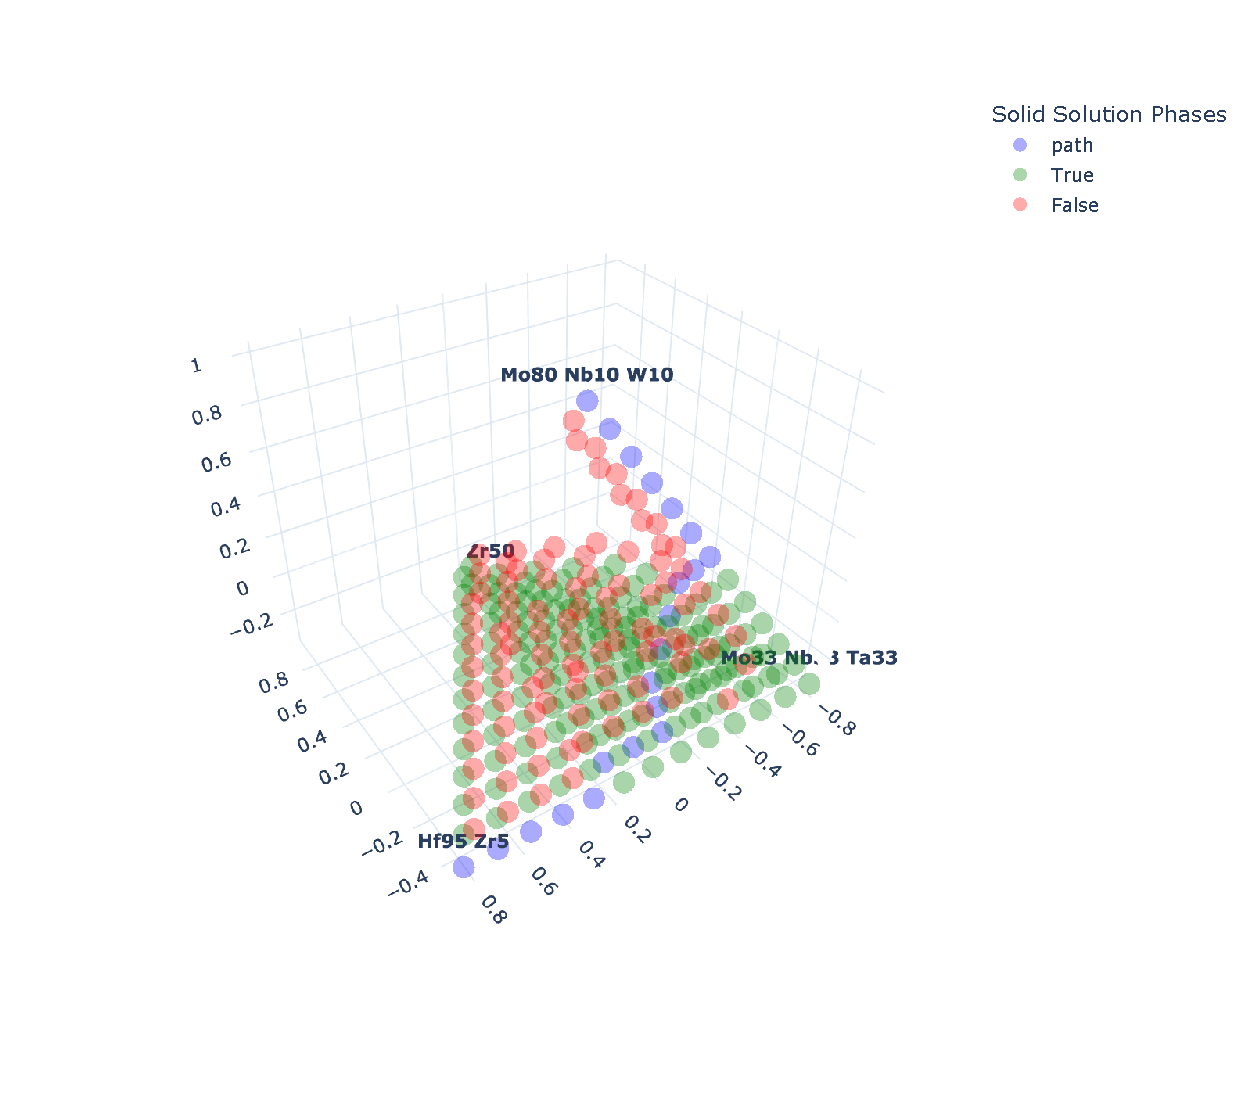
\includegraphics[width=0.8\textwidth]{nimplextutorial2/02.AdditiveManufacturingPathPlanning_65_1.pdf}
    \caption{An biased selection from a set of equally optimal shortest paths between W10 Nb10 Mo80 and Ti5 Hf95 connecting them in 21 steps, penalized by the magnitude of gradient of RMSAD over the path. Relative to one in Figure \ref{nimplextutorial2:fig:shortest}, it passes closer to the center of the compositional space to avoid low-RMSAD region around MoNbTa and possibly pass through iso-value surface. It can also be seen as the shortest path in a stretched space.}
    \label{nimplextutorial2:fig:lowgradient}
\end{figure}


\section{Property Maximization Along the
Path}\label{nimplextutorial2:property-maximization-along-the-path}

\textbf{Finally, let's demonstrate how easy it is to maximize a property
along the path by exploiting the unidirectionaliy of the graph edge
definitions in \texttt{nimplex}, which allow us to
efortlessly enocde the property maximization goal as directional reward
or penalty applied to edges.} This is as simple as applying the property
gradient directly rather than its magnitude.

\begin{minted}[breaklines, xleftmargin=3\parindent, linenos=true, fontsize=\small]{python}
edges = []
gradientsList = []
penaltyFactor = 20
for i, nList in enumerate(graphN):
    if gridFeasible[i]:
        for n in nList:
            if gridFeasible[n]:
                rmsadGradient = rmsadList[i]-rmsadList[n]
                gradientsList.append(rmsadGradient)
                edges.append([i, n, 1+round((rmsadGradient*penaltyFactor), 3)])
print(edges[:15])
print(f"{len(gradientsList)} gradients calculated with values up to {max(gradientsList)}")
print(f"Penalty at -{penaltyFactor}x gradient *value* per path step assigned (higher RMSAD preferred)")
\end{minted}

\begin{minted}[xleftmargin=3\parindent, fontsize=\small, bgcolor=subtlegray]{output}
[[0, 1, 0.945], [1, 0, 1.055], [1, 2, 0.954], [2, 1, 1.046], [2, 3, 0.958], 
[3, 2, 1.042], [3, 4, 0.961], [4, 3, 1.039], [4, 5, 0.962], [5, 4, 1.038], 
[5, 6, 0.963], [6, 5, 1.037], [6, 7, 0.963], [6, 97, 0.577], [7, 6, 1.037]]
1374 gradients calculated with values up to 0.0473823732310002
Penalty at -20x gradient *value* per path step assigned (higher RMSAD preferred)
\end{minted}

\begin{minted}[xleftmargin=3\parindent, linenos=true]{python}
pathfindingGraph = Graph(edges=edges, bi_directional=False)
finder = DijkstraFinder()
path, runs = finder.find_path(
    pathfindingGraph.node(0), 
    pathfindingGraph.node(90), 
    pathfindingGraph)
pathList = [p.node_id for p in path]
\end{minted}

\begin{minted}[breaklines, xleftmargin=3\parindent, linenos=true, fontsize=\small]{python}
for step, i in enumerate(pathList):
    print(f"{step+1:>2}: {formulas[i]}")
\end{minted}

\begin{minted}[xleftmargin=3\parindent, fontsize=\small, bgcolor=subtlegray]{output}
 1: (  0) W10.0 Nb10.0 Mo80.0 
 2: (  1) W11.9 Nb11.9 Ta2.8 Mo73.3 
 3: (  2) W13.9 Nb13.9 Ta5.6 Mo66.7 
 4: (  3) W15.8 Nb15.8 Ta8.3 Mo60.0 
 5: (  4) W17.8 Nb17.8 Ta11.1 Mo53.3 
 6: (  5) W19.7 Nb19.7 Ta13.9 Mo46.7 
 7: (  6) W21.7 Nb21.7 Ta16.7 Mo40.0 
 8: ( 97) Ti4.2 Zr4.2 W20.8 Nb20.8 Ta16.7 Mo33.3 
 9: (175) Ti8.3 Zr8.3 W20.0 Nb20.0 Ta16.7 Mo26.7 
10: (186) Ti8.8 Zr8.3 Hf7.9 W19.2 Nb19.2 Ta16.7 Mo20.0 
11: (196) Ti9.2 Zr8.3 Hf15.8 W18.3 Nb18.3 Ta16.7 Mo13.3 
12: (204) Ti9.6 Zr8.3 Hf23.8 W15.6 Nb15.6 Ta13.9 Mo13.3 
13: (212) Ti10.0 Zr8.3 Hf31.7 W14.7 Nb14.7 Ta13.9 Mo6.7 
14: (219) Ti10.4 Zr8.3 Hf39.6 W13.9 Nb13.9 Ta13.9 
15: (153) Ti6.7 Zr4.2 Hf47.5 W13.9 Nb13.9 Ta13.9 
16: (158) Ti7.1 Zr4.2 Hf55.4 W11.1 Nb11.1 Ta11.1 
17: (162) Ti7.5 Zr4.2 Hf63.3 W8.3 Nb8.3 Ta8.3 
18: (165) Ti7.9 Zr4.2 Hf71.2 W5.6 Nb5.6 Ta5.6 
19: (167) Ti8.3 Zr4.2 Hf79.2 W2.8 Nb2.8 Ta2.8 
20: (168) Ti8.8 Zr4.2 Hf87.1 
21: ( 90) Ti5.0 Hf95.0 
\end{minted}

\textbf{As you can see, we again complete the path in 21 steps but
following a different path that maximizes the RMSAD along the way thanks
to the small bias we introduced.}

\begin{minted}[breaklines, xleftmargin=3\parindent, linenos=true, fontsize=\small]{python}
gridFeasibleMarked = ['path' if i in pathList else f for i, f in enumerate(gridFeasible)]
fig = px.scatter_3d(
  gridAtt_projected_df, x='x', y='y', z='z', color=gridFeasibleMarked, 
  text=labels, hover_name=formulas, template='plotly_white', width=800, 
  height=700, opacity=0.333, color_discrete_sequence=['blue', 'green', 'red'], 
  labels={'color':'Solid Solution Phases', 'x':'', 'y':'', 'z':''})
fig.update_scenes({'camera': {'eye': {'x': -1.8, 'y': 1.2, 'z': 1.5}}})
\end{minted}

\begin{figure}[H]
    \centering
    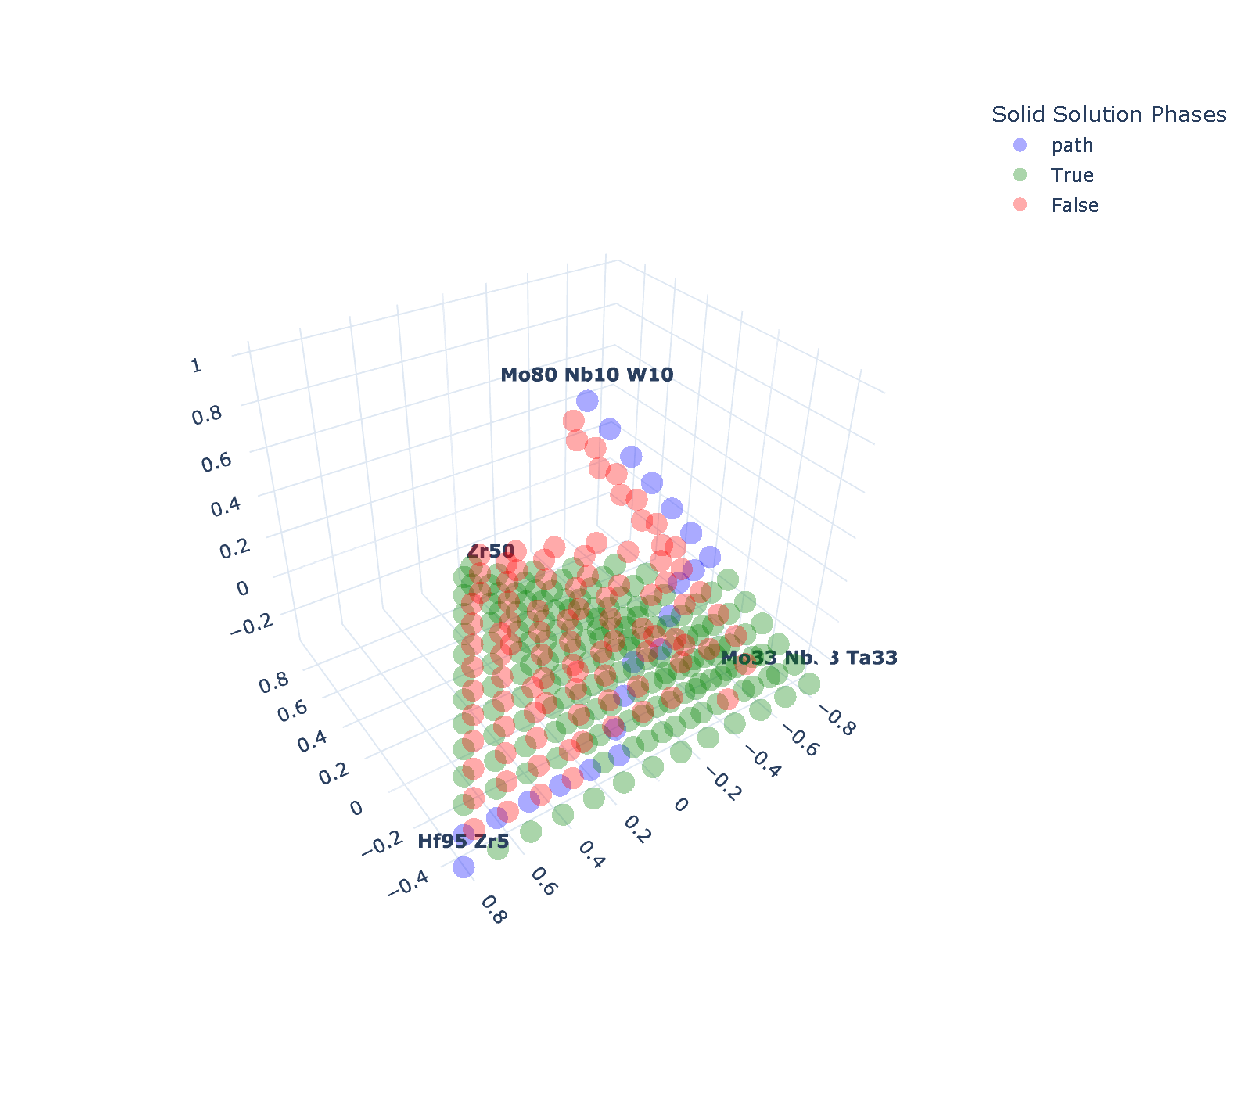
\includegraphics[width=0.8\textwidth]{nimplextutorial2/02.AdditiveManufacturingPathPlanning_71_1.pdf}
    \caption{An biased selection from a set of equally optimal shortest paths between W10 Nb10 Mo80 and Ti5 Hf95 connecting them in 21 steps, penalized for negative the value of gradient of RMSAD over the path. It can also be seen as the shortest path in a bidirectionally stretched space.}
    \label{nimplextutorial2:fig:highvalue}
\end{figure}


\textbf{And, if we care more about going through high RMSAD regions than
we do about the number of steps taken, we can always simply increase the
bias to move the path into the high RMSAD regions even more at the cost
of the number of steps taken.}

\begin{minted}[breaklines, xleftmargin=3\parindent, linenos=true, fontsize=\small]{python}
edges = []
gradientsList = []
penaltyFactor = 200
for i, nList in enumerate(graphN):
    if gridFeasible[i]:
        for n in nList:
            if gridFeasible[n]:
                rmsadGradient = rmsadList[i]-rmsadList[n]
                gradientsList.append(rmsadGradient)
                edges.append([i, n, 1+round((rmsadGradient*penaltyFactor), 3)])
print(edges[:15])
print(f"{len(gradientsList)} gradients calculated with values up to {max(gradientsList)}")
print(f"Penalty at -{penaltyFactor}x gradient *value* per path step assigned (higher RMSAD preferred)")

pathfindingGraph = Graph(edges=edges, bi_directional=False)
finder = DijkstraFinder()
path, runs = finder.find_path(
    pathfindingGraph.node(0), 
    pathfindingGraph.node(90), 
    pathfindingGraph)
pathList = [p.node_id for p in path]
\end{minted}

\begin{minted}[xleftmargin=3\parindent, fontsize=\small, bgcolor=subtlegray]{output}
[[0, 1, 0.44599999999999995], [1, 0, 1.554], [1, 2, 0.536], [2, 1, 1.464], 
[2, 3, 0.5840000000000001], [3, 2, 1.416], [3, 4, 0.609], [4, 3, 1.391], 
[4, 5, 0.621], [5, 4, 1.379], [5, 6, 0.625], [6, 5, 1.375], [6, 7, 0.626], 
[6, 97, -3.2300000000000004], [7, 6, 1.374]]
1374 gradients calculated with values up to 0.0473823732310002
Penalty at -200x gradient *value* per path step assigned (higher RMSAD preferred)
\end{minted}

\begin{minted}[breaklines, xleftmargin=3\parindent, linenos=true, fontsize=\small]{python}
for step, i in enumerate(pathList):
    print(f"{step+1:>2}: {formulas[i]}")
\end{minted}

\begin{minted}[xleftmargin=3\parindent, fontsize=\small, bgcolor=subtlegray]{output}
1: (  0) W10.0 Nb10.0 Mo80.0 
 2: (  1) W11.9 Nb11.9 Ta2.8 Mo73.3 
 3: (  2) W13.9 Nb13.9 Ta5.6 Mo66.7 
 4: (  3) W15.8 Nb15.8 Ta8.3 Mo60.0 
 5: (  4) W17.8 Nb17.8 Ta11.1 Mo53.3 
 6: (  5) W19.7 Nb19.7 Ta13.9 Mo46.7 
 7: (  6) W21.7 Nb21.7 Ta16.7 Mo40.0 
 8: ( 97) Ti4.2 Zr4.2 W20.8 Nb20.8 Ta16.7 Mo33.3 
 9: (175) Ti8.3 Zr8.3 W20.0 Nb20.0 Ta16.7 Mo26.7 
10: (186) Ti8.8 Zr8.3 Hf7.9 W19.2 Nb19.2 Ta16.7 Mo20.0 
11: (196) Ti9.2 Zr8.3 Hf15.8 W18.3 Nb18.3 Ta16.7 Mo13.3 
12: (205) Ti9.6 Zr8.3 Hf23.8 W17.5 Nb17.5 Ta16.7 Mo6.7 
13: (213) Ti10.0 Zr8.3 Hf31.7 W16.7 Nb16.7 Ta16.7 
14: (219) Ti10.4 Zr8.3 Hf39.6 W13.9 Nb13.9 Ta13.9 
15: (279) Ti14.6 Zr12.5 Hf39.6 W11.1 Nb11.1 Ta11.1 
16: (328) Ti18.8 Zr16.7 Hf39.6 W8.3 Nb8.3 Ta8.3 
17: (367) Ti22.9 Zr20.8 Hf39.6 W5.6 Nb5.6 Ta5.6 
18: (369) Ti23.3 Zr20.8 Hf47.5 W2.8 Nb2.8 Ta2.8 
19: (333) Ti19.6 Zr16.7 Hf55.4 W2.8 Nb2.8 Ta2.8 
20: (288) Ti15.8 Zr12.5 Hf63.3 W2.8 Nb2.8 Ta2.8 
21: (233) Ti12.1 Zr8.3 Hf71.2 W2.8 Nb2.8 Ta2.8 
22: (167) Ti8.3 Zr4.2 Hf79.2 W2.8 Nb2.8 Ta2.8 
23: (168) Ti8.8 Zr4.2 Hf87.1 
24: ( 90) Ti5.0 Hf95.0 
\end{minted}


\begin{minted}[breaklines, xleftmargin=3\parindent, linenos=true, fontsize=\small]{python}
gridFeasibleMarked = ['path' if i in pathList else f for i, f in enumerate(gridFeasible)]
fig = px.scatter_3d(
  gridAtt_projected_df, x='x', y='y', z='z', color=gridFeasibleMarked, 
  text=labels, hover_name=formulas, template='plotly_white', width=800, 
  height=700, opacity=0.333, color_discrete_sequence=['blue', 'green', 'red'],
  labels={'color':'Solid Solution Phases', 'x':'', 'y':'', 'z':''})
fig.update_scenes({'camera': {'eye': {'x': -1.8, 'y': 1.2, 'z': 1.5}}})
\end{minted}

\begin{figure}[H]
    \centering
    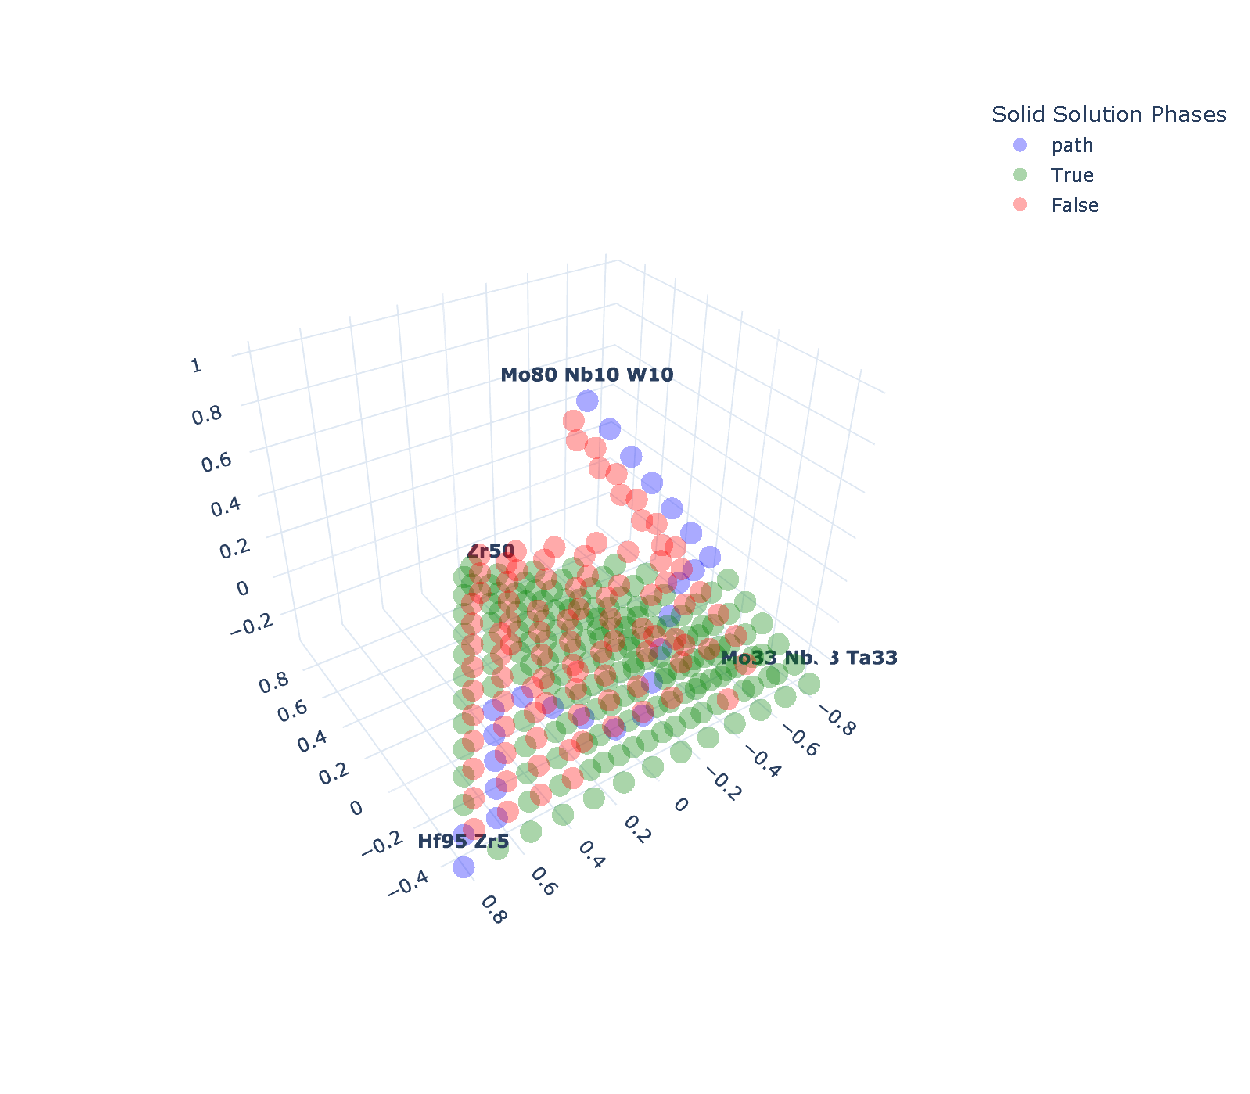
\includegraphics[width=0.8\textwidth]{nimplextutorial2/02.AdditiveManufacturingPathPlanning_74_1.pdf}
    \caption{A paths between W10 Nb10 Mo80 and Ti5 Hf95, connecting them in 24 steps, very strongly biased towards regions of high RMSAD.}
    \label{nimplextutorial2:fig:veryhighvalue}
\end{figure}

\section{Final Remarks} \label{nimplextutorial2:final-remarks}

\textbf{And that's it! We hope you enjoyed this tutorial and that you
see the potential of \texttt{nimplex} in your work. If
you have any questions, feel free to ask them in the
\texttt{nimplex} repository under the Issues tab. You
are also welcome to shoot an email to the author at
\href{mailto:adam@phaseslab.org}{\nolinkurl{adam@phaseslab.org}}. We
will be excited to hear about your applications.}